\section{Memory flatenig}

A common problem in multidimensional data situations is memory layout representation. Internally computers always represnt memorry in a linear fashion, the idea of mutidimensional array is just sugar syntax added by high level programming lenguajes.

Given said that, sometimes such allocations can become dificult to use or declare by themselves. Especially in C++. Lets see an example:

{\centering
\begin{minipage}{\linewidth}
  \begin{listing}[H]
  \inputminted[
  xleftmargin=1.5cm,  %without this option line number goes wrong
  %frame=lines,
  framesep=0.5cm,
  baselinestretch=1.2,
  %fontsize=\footnotesize,
  linenos,
  firstline=15, %If you omit this two fields, the whole file is pulled
  lastline=21
  ]{cpp}{src/ArrayDimensions.cpp}
  \caption{One dimensioal array (by means of \mintinline{cpp}{std::vector} class) used}
  \label{lst:1Dexample}
  \end{listing}
\end{minipage}
\par
}
\vspace{0.5cm}
So far, everything looks good, sintax is clear, braket operator is helping us. 
Conceptually, we have a series of variables with the same type that live in a contiguos space in memory. See figure~\ref{fig:1D}.

\begin{figure}[htp]
  \centering
  \begin{subfigure}[b]{0.35\textwidth}
    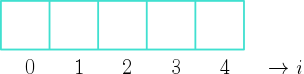
\includegraphics[width=\textwidth]{img/array1D}
    \caption{Logical memory layout representation.}
  \label{fig:1a}
  \end{subfigure}
  \hspace*{4cm}
  \begin{subfigure}[b]{0.25\textwidth}
    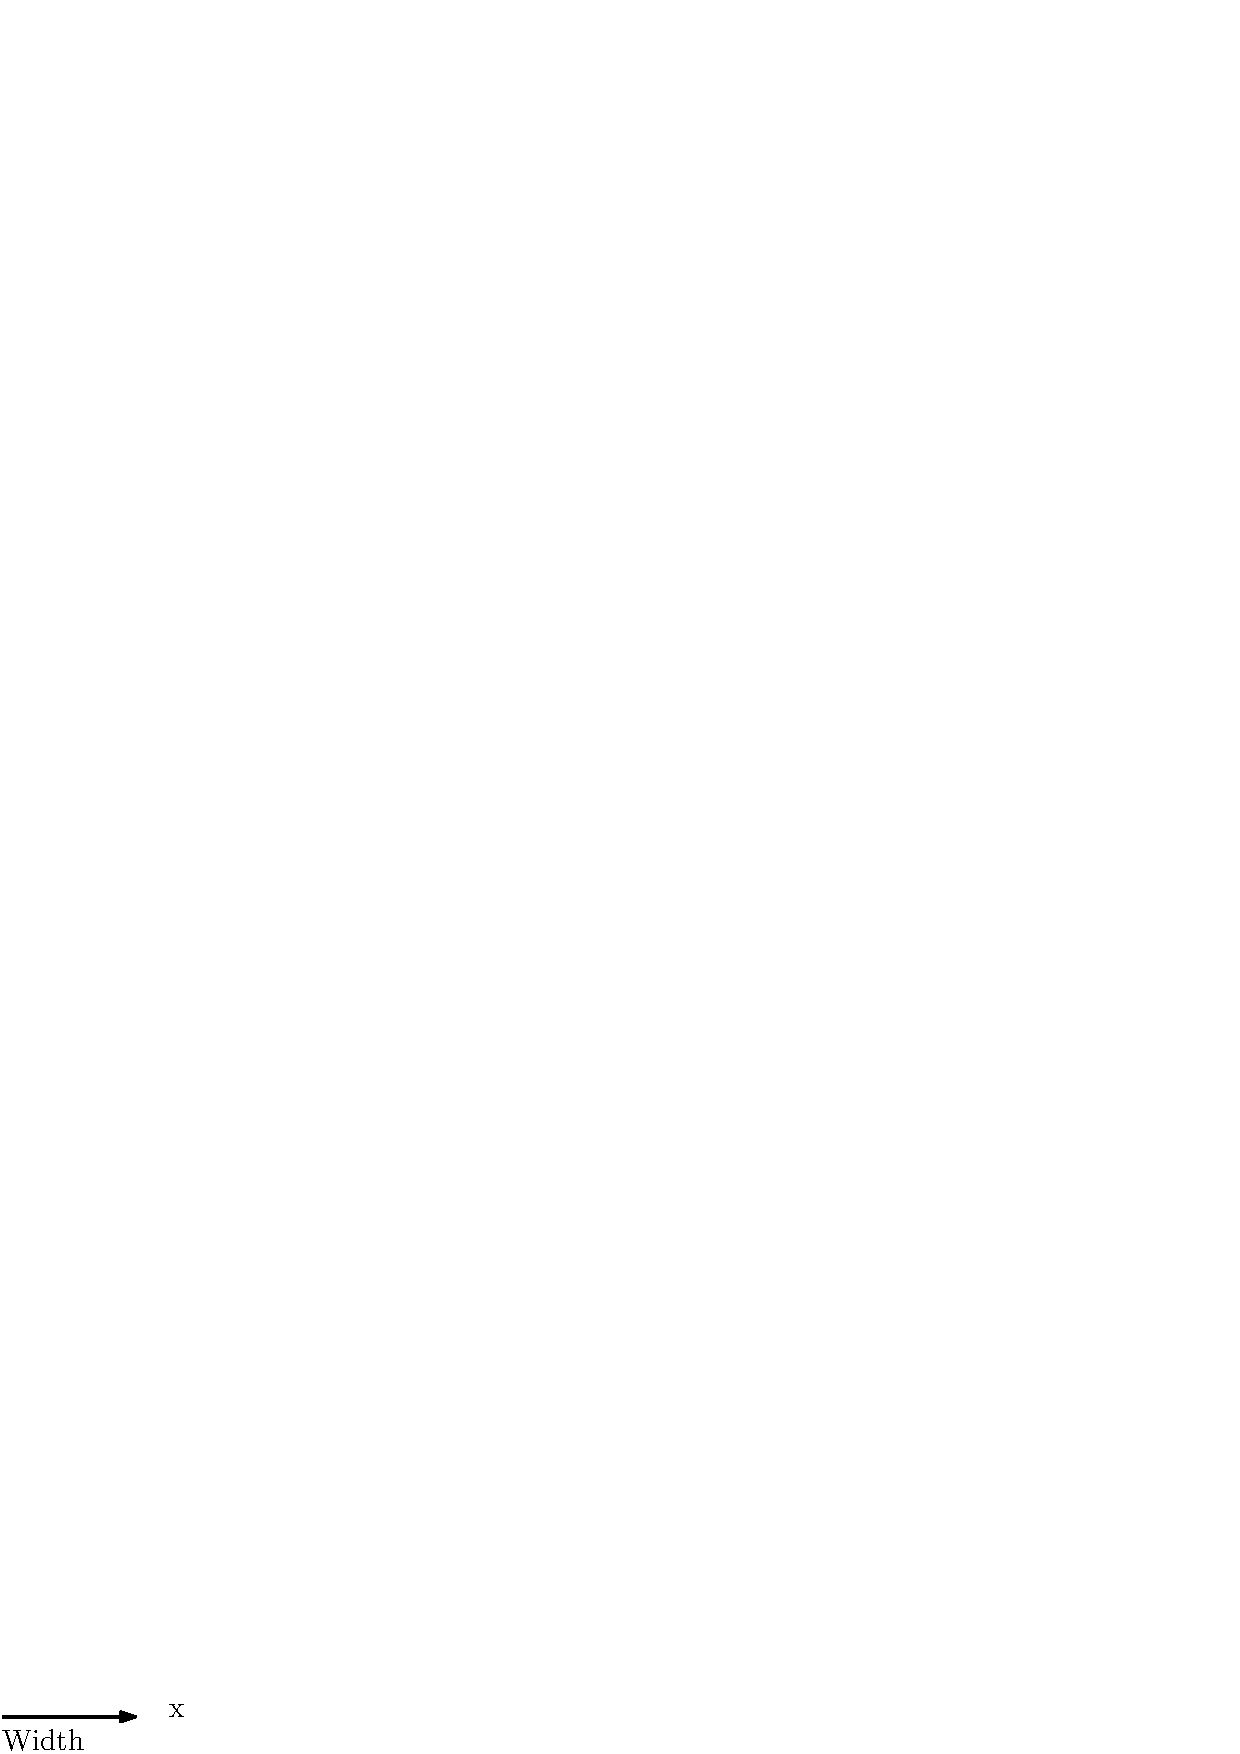
\includegraphics[width=\textwidth]{img/arrow1D}
    \caption{Dimensions represented.}
    \label{fig:1b}
  \end{subfigure}
  \caption{One dimensional array representation.}
  \label{fig:1D}
\end{figure}

The problem becomes evident as data start to include more dimensions. 
In a bidimensional array we have data that has two dimensions.
One can think about it like data it's in a table, the situation is the one depicted in Figure~\ref{fig:2a}. 
Now, remember this is just an abstraction (provided by our programming language: C++; in this case), since memory is actually \emph{close} to linear in a computer.

\begin{figure}[htp]
  \centering
  \begin{subfigure}[b]{0.35\textwidth}
    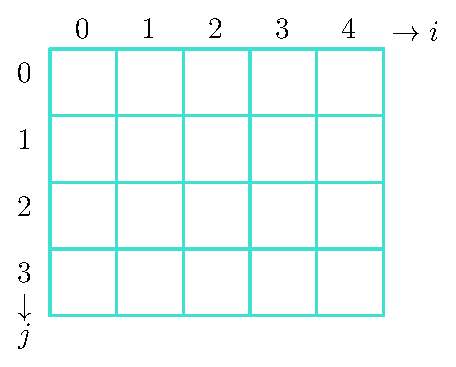
\includegraphics[width=\textwidth]{img/array2D}
    \caption{Logical memory layout representation.}
  \label{fig:2a}
  \end{subfigure}
  \hspace*{4cm}
  \begin{subfigure}[b]{0.25\textwidth}
    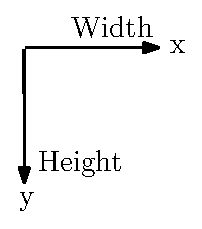
\includegraphics[width=\textwidth]{img/arrow2D}
    \caption{Dimensions represented.}
    \label{fig:2b}
  \end{subfigure}
  \caption{Two dimensional array representation.}
  \label{fig:2D}
\end{figure}

Usually, the C++ way of modeling this is creating an array, such that each element of it, is also an array. See the code in Listing~\ref{lst:2dexample}

{\centering
\begin{minipage}{\linewidth}
  \begin{listing}[H]
  \inputminted[
  xleftmargin=1.5cm,  %without this option line number goes wrong
  %frame=lines,
  framesep=0.5cm,
  baselinestretch=1.2,
  %fontsize=\footnotesize,
  linenos,
  firstline=23, %If you omit this two fields, the whole file is pulled
  lastline=38
  ]{cpp}{src/ArrayDimensions.cpp}
  \caption{Two dimensioal array example}
  \label{lst:2dexample}
  \end{listing}
\end{minipage}
\par
}
\vspace{0.5cm}
Now, there is two main points to highlight in the sample:
\begin{enumerate}

\item The type of the array has change. 
      Now is \emph{a vector of int vectors}.
      This led us to have a longer initialization for it too.
      Imagine that you create functions to receive or return such arrays.
      The sintax to declare the parameters become difficult.

 \item We still have the advantage of a very elegant sintax to use the array: \mintinline{cpp}{b[j][i]} give us the element on column $i$ of row $j$ (we are zero based).

 \end{enumerate}
 
Here is when the technique called \emph{memory flattening} becomes useful.
In simple words: This is to mimic what the compiler is doing for us: use linear data. 
But at the same time you also provide an abstraction, so you can access it in a similar fashion that if your data had more dimensions.
In other works you simulate the access via indices for all the simulated dimensions.

This has the advantage that all the data is store in a one dimensional array.
Therefore, you \emph{ensure} all your data is actually contigous in memory.
Also, no matter how many dimensions your data has, the type is always a one dimensional array.
Finally, due \emph{cache} issues, the access tends to be faster than the alternative.

Now is clear, that in order to implement this technique we will need two mappings:
First, a function $g:\mathbb{Z}^n \rightarrow \mathbb{Z}$, to map the indices in $n$ dimensions to the one dimensional array.
And second, the inverse mapping $h:\mathbb{Z} \rightarrow \mathbb{Z}^n$ to retrive the indices back given a position in the data buffer.

Let's see this idea for the 2D case.
Assume that our data hast two dimensions ($x$ and $y$ --or \emph{width} and \emph{height}-- if you like).
That we use two indices $i$ and $j$ to transverse it.
And assume also that the maximun values of such indices are \mintinline{cpp}{WIDTH} and \mintinline{cpp}{HEIGHT} and that they are zero based.
See the Figure~\ref{fig:2D}.

The first function $g$ it is actually the most useful to us, since it will provide with the interface of accesing our data. 
In Listing~\ref{lst:functions2D} we show the implementation of such function.
We can see that the transformations are actully very simple.
In fact one of them is the integer division and the other one is a modulo.
Also note, that as long as we check for the boundaries of the values for both indices, only one of the maximun dimensions in this case \emph{witdh} is used in the actual calculation of the indices.

{\centering
\begin{minipage}{\linewidth}
  \begin{listing}[H]
  \inputminted[
  xleftmargin=1.5cm,  %without this option line number goes wrong
  %frame=lines,
  framesep=0.5cm,
  baselinestretch=1.2,
  %fontsize=\footnotesize,
  linenos,
  firstline=86, %If you omit this two fields, the whole file is pulled
  lastline=103
  ]{cpp}{src/FlatMemmory.cpp}
  \caption{Function $g$ to map real index into simulated 2D indices}
  \label{lst:functions2D}
  \end{listing}
\end{minipage}
\par
}
\vspace{0.5cm}

For completeness, we also show Listing~\ref{lst:functions2D2} that defines the inverse function $h$, to retrive the index in the one dimensional array from the two simulated indices in 2D.

{\centering
\begin{minipage}{\linewidth}
  \begin{listing}[H]
  \inputminted[
  xleftmargin=1.5cm,  %without this option line number goes wrong
  %frame=lines,
  framesep=0.5cm,
  baselinestretch=1.2,
  %fontsize=\footnotesize,
  linenos,
  firstline=105, %If you omit this two fields, the whole file is pulled
  lastline=119
  ]{cpp}{src/FlatMemmory.cpp}
  \caption{Function $h$ to map simulated 2D indices into the real index, this is the inverse of $g$}
  \label{lst:functions2D2}
  \end{listing}
\end{minipage}
\par
}
\vspace{0.5cm}

Now, lets look at the more complex --but still very common-- scenario of three dimensions. The situation is the one depicted in Figure~\ref{fig:3D}. We include a new dimension of in the data,

\begin{figure}[htp]
  \centering
  \begin{subfigure}[b]{0.35\textwidth}
    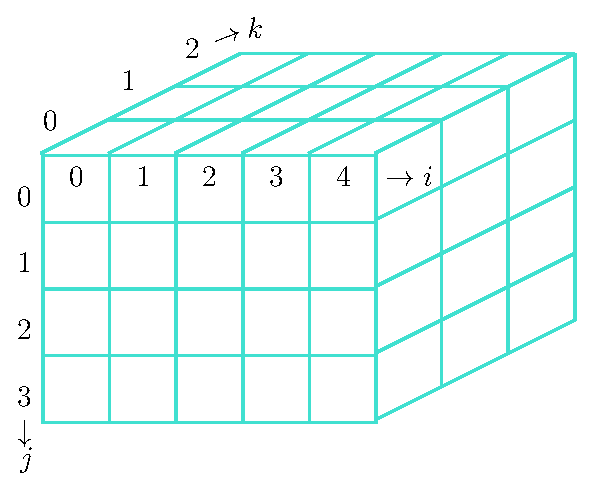
\includegraphics[width=\textwidth]{img/array3D}
    \caption{Logical memory layout representation.}
  \label{fig:3a}
  \end{subfigure}
  \hspace*{4cm}
  \begin{subfigure}[b]{0.2\textwidth}
    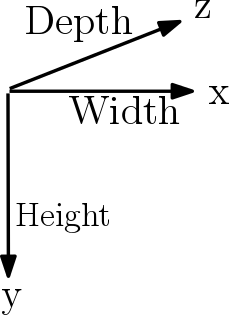
\includegraphics[width=\textwidth]{img/arrow3D}
    \caption{Dimensions represented.}
    \label{fig:3b}
  \end{subfigure}
  \caption{Three dimensional array representation.}
  \label{fig:3D}
\end{figure}

\section{Bitwise operation}
\begin{itemize}
  \item Basic operations. Bit vs Byte How to handle printing in C++
  \item One bit manipulation, set, clear, toggle and testing
  \item Bit masking: set, clear, toggle and test group of bites
\end{itemize}

\section{Analytic Geometry}
\begin{itemize}
  \item Ray, line and segment representations
  \item Ray to segment intersection
  \item Projecction
  \item Point to segment distance
  \item Belonging test on simple polygons
\end{itemize}

\section{Graphics Pipeline}
\begin{itemize}
  \item Simple: Vertex and fragment
  \item Complete, all optional stages
  \item Texture pipeline
\end{itemize}
